\documentclass{VUMIFPSkursinis}
\usepackage{hyperref}
\usepackage{algorithmicx}
\usepackage{algorithm}
\usepackage{algpseudocode}
\usepackage{amsfonts}
\usepackage{amsmath}
\usepackage{bm}
\usepackage{caption}
\usepackage{color}
\usepackage{float}
\usepackage{graphicx}
\usepackage{listings}
\usepackage{subcaption}
\usepackage{wrapfig}
\usepackage{biblatex}
\setcounter{tocdepth}{3}

\university{Vilniaus universitetas}
\faculty{Matematikos ir informatikos fakultetas}
\institute{Informatikos institutas}
\department{Programų sistemų studijų programa}
\papertype{Kursinis darbas}
\title{Interneto programų išleidimo valdymas naudojant laikinąsias aplinkas}
\titleineng{Release management of Web Applications using temporary environments}
\status{4 kurso 1 grupės studentas}
\author{Domas Pozniakas}
\supervisor{lekt. Aurimas Šimkus}
\date{Vilnius – \the\year}

\bibliography{bibliografija}

\begin{document}
\maketitle

\tableofcontents

\sectionnonum{Įvadas}
Šių dienų pasaulyje visa mūsų aplinka ir gyvenimas tiesiogiai priklauso nuo IT kuriamų sprendimų. Kompanijos skiria savo laiką internetinių programų vystymui, taip pat ir procesams susijusiems su sukurtos programinės įrangos išleidimu (angl. \textit{release}). Kitu atveju, paruošti leidimai nėra pateikiami klientui tinkamai ir jie susiduria su nemažai problemų, nors pats produktas ir yra kokybiškas. Visos šios situacijos vis labiau iškelia efektyvų programinės įrangos išleidimo valdymo poreikį. Atkreipiama daugiau dėmesio į internetinių programų kūrimo, testavimo ir diegimo valdymo procesus, kuriuose išryškėja tokių veiklų svarba, kaip skirtingų komandų darbo koordinavimas, išleidimo datų planavimas, programinės įrangos testavimo ir paruošimo diegimui užtikrinimas. Tačiau daugelyje įmonių su pastarosiomis pora veiklų kyla nemažai problemų, nepaisant visų turimų būtinųjų išteklių (t.y. tokių, kaip žmogiškieji, finansiniai bei laiko ištekliai), nes trūksta efektyvaus valdymo susijusio su programinės įrangos išleidimu \cite{SaltPirmas}. 


Vienas iš alternatyvių ir dar nespėjusių plačiai išpopuliarėti būdų suvaldyti programinės įrangos išleidimo procesus internetinėms programoms yra naudoti laikinas aplinkas, kurios yra izoliuotos, naudojamos testavimui ir diegimui. Šios aplinkos leidžia komandoms išbandyti naujus programinės įrangos leidimus nepažeidžiant produkcinės (angl. \textit{production}) aplinkos, kurioje internetine svetaine jau naudojasi klientai \cite{SaltAntras}. Tai suteikia galimybes laisviau ir geriau testuoti naujus funkcionalumus, kadangi nėra grėsmės pažeisti jautrių duomenų, sutrikdyti klientų patirties ar kolegų darbo efektyvumo. Tačiau daugeliui įmonių reikia atsargiai vertinti galimybę įgyvendinti ir automatizuoti tokią metodiką. Remiantis 2011 metais atlikto tyrimo duomenimis - daug įmonių teigia, kad trūksta visapusiškų įrankių, kurie leistų ir padėtų automatizuoti procesus susijusius su programinės įrangos išleidimo valdymu \cite{SaltPirmas}. Dėl šių priežasčių laikinųjų aplinkų paruošimas ir priežiūra gali atimti nemažai laiko sąnaudų ir brangiai kainuoti.

 Atsižvelgiant į tai, kad siekiant įgyvendinti šią metodiką kyla nemažai galimų rizikų ar sunkumų - darbe siekiama nustatyti ar laikinosios aplinkos yra tinkamas ir efektyvus sprendimas, norint pagerinti programuotojų, testuotojų ir kitų profesijų, susijusių su IT sektoriumi, patirtį bei produkto sėkmingo veikimo rezultatus. Tam reikia turėti gerai funkcionuojančius programinės įrangos išleidimo valdymo procesus, kurie suteiktų galimybę tinkamai testuoti, apsaugoti ir užtikrinti stabilų produkto veikimą produkcinėje aplinkoje. Taip pat, integruoti vieną iš rekomenduojamų sprendimų praktiškai bei palyginti su tradiciniais būdais programinės įrangos išleidimo valdyme.

\bigskip

\textbf{Darbo tikslas} - įvertinti laikinųjų aplinkų interneto programoms tinkamumą išleidimo valdymui. 

\textbf{Darbe keliami uždaviniai:}

1. Išanalizuoti tradicinius programinės įrangos išleidimo internetinėms programoms būdus.

2. Apžvelgti laikinų aplinkų sprendimą tokio tipo sistemoms bei jo taikymą.

3. Integruoti rekomendacinį laikinųjų aplinkų sprendimą į programinės įrangos išleidimo valdymą.

% 1 dalis. Tradciniai metodai
\section{Tradicinių išleidimo valdymo metodikų apžvalga}
Šiame skyriuje nagrinėjama teorinė medžiaga apie įprastas programinės įrangos išleidimo valdymo metodikas, įskaitant ir naudojamas praktikas bei principus, kurie taikomi ruošiant sukurto IT sprendimo leidimus į produkcinę aplinką. Tikslas yra suteikti skaitytojui geresnį suvokimą apie šią sritį ir su kokiomis problemomis IT sektoriuje yra susiduriama taikant įprastus valdymo metodus šiuo metu.

\subsection{Pagrindiniai principai}
Kuriant programinę įrangą ir valdant jos leidimus, susiformavo keli esminiai principai ir nepriklausomai nuo kitų aplinkybių, jie yra naudojami planuojant, kontroliuojant bei vykdant programinės įrangos išleidimo procesus. Juos visus galima patalpinti į Krioklio (angl. \textit{Waterfall}) metodą, kurį sudaro penkios dalys \cite{SaltTrecias}.

\begin{figure}[H]
    \centering
    \includegraphics[scale=0.5]{img/WaterfallLT2.png}
    \caption{Krioklio metodo schema}
    \label{img:mlp}
\end{figure}

Šis metodas yra taip pavadintas, kadangi jo veikimo principo pavaizdavimas yra paremtas tradiciniais pramoniniais vamzdynais, kur viskas vyksta aiškiai apibrėžtais etapais ir eiliškumu \cite{SaltTrecias}. Kiekvienas iš šio metodo etapų atitinka konkretų principą susiformavusį IT sektoriuje:

\begin{itemize}
    % TODO: Suinteresuotos šalys - įdėti į sąvokas
  \item \textit{Reikalavimai}. Svarbu gauti tikslius poreikius iš klientų ir kitų suinteresuotų šalių (išlaikant pakankamai aukštą abstrakcijos lygį, kad būtų galima juos tobulinti sekančiuose Krioklio metodo etapuose). Formuojant reikalavimus taip pat atsižvelgiama į turimus resursus bei ar dokumentuoti reikalavimai atitinka verslo strategiją \cite{SaltKetvirtas}. Taip yra užtikrinama, kad kliento lūkesčiai ir verslo kryptis bus teisinga, kai kiekvienas iš poreikių bus tiksliai suformuluotas bei įgyvendintas. Iš anksto apsisaugojus nuo galimų nesusipratimų tarp užsakovo ir vykdytojo yra išvengiama dalies problemų, kurios atsirastų naujam leidimui patekus į produkcinę aplinką.

  \item \textit{Projektavimas}. Proceso metu bandoma suprojektuoti sistemos architektūrą, kuri vėliau yra patikrinama siekiant įsitikinti ar nėra nukrypimų nuo reikalavimų, turimų resursų bei produkto apimties \cite{SaltKetvirtas}. Suformuota architektūra leidžia iš anksto numatyti galimas problemas ir turėti stabiliai veikiančią sistemą išvengiant projektavimo bei optimizavimo klaidų atsiradus naujiems leidimams, kurie keičia sistemos veikimą. 
  
  \item \textit{Implementacija}. Programinė įranga kuriama pagal suformuotus reikalavimus, kurie buvo paruošti ankstesniuose etapuose \cite{SaltPenktas}.  Autoriaus nuomone tai leidžia išvengti komunikacijos klaidų tarp klientų, suinteresuotų šalių ir vykdytojų. O tai lemia, kad programinė įranga yra išleidžiama dažniau į produkcinę aplinką mažesniais komponentais arba vienetais, nes nėra reikalingas pilnai įgyvendintas funkcionalumas, kuris leistų įsitikinti ar tai atitinka kliento poreikius.
  
  \item \textit{Verifikacija}. Šiam principui užtikrinti reikalinga testuotojų komanda, kuri prieš išleidžiant naujus leidimus tikrina naujo kodo kokybę bei paruoštus funkcionalumus \cite{SaltKetvirtas}. Tai leidžia nustatyti, ar sistema yra paruošta naudotis klientams ir galima dislokuoti naują leidimą.
  
  \item \textit{Priežiūra}. Laikomasi principo, kad jei klientai susiduria su problemomis, kurios susijusios su teikiama programine įranga - jie gali apie jas pranešti atsakingiems asmenims ir gauti pagalbą siekiant jas išspręsti \cite{SaltKetvirtas}. Jei atrandamos problemos programinėje įrangoje - grįžtama į implementacijos etapą ir praėjus visus žingsnius yra paruošiamas naujas leidimas, kuris išsprendžia klientui atsiradusias problemas.
\end{itemize}

Griežta programinės įrangos išleidimo etapų struktūra leidžia užtikrinti, kad sistema veiktų tinkamai, nes tarp visų etapų dokumentai praeina kokybės patikrą, o juose saugoma tokia informacija kaip kliento reikalavimai, turimi resursai ar sistemos architektūra \cite{SaltKetvirtas}. Tačiau naudojant šį metodą visas procesas vyksta sinchroniškai, todėl nukenčia naujų funkcionalumų trukmė iki kol jie atsidurs produkcinėje aplinkoje. Krioklio metodas neišpildo visų internetinių programų poreikių, nes jis skirtas labiau programinei įrangai, kurios leidimai būna milžiniški ir yra išleidžiami vos kelis kartus per metus ar dar rečiau \cite{SaltTrecias}.

% TODO: PĮ įtraukti į Santrumpas
% TODO: Sužiūrėti visur angliškų lietuviškų žodžių reikšmes(Pvz.: ar Iteracija = Sprint)
\subsection{„Agile“ principai PĮ išleidimo valdyme}

Šios metodikos pagrindinės idėjos plačiai naudojamos įvairiose IT srityse - ne išimtis ir programinės įrangos išleidimo valdyme. Autoriaus nuomone „Agile“ principai yra sunkiai išvengiami įmonėms, norinčioms užtikrinti stabilų funkcionalumų pristatymą, nuolatinį testavimą ir lankstumą keistis. PĮ leidimų valdyme ši metodika gali būti taikoma produktų leidimų kūrimui, testavimui ir diegimui valdyti. Tai apima kūrimo proceso padalijimą į mažesnius, iteracijų (angl. \textit{Sprint}) ciklus, kurie leidžia geriau planuoti mažus leidimus. „Agile“ taip pat išpildo ir prieš tai aptartų pagrindinių principų idėją, kad reikia glaudžiai bendradarbiauti su suinteresuotosiomis šalimis, kadangi reikia nustatyti funkcijų prioritetus ir prireikus atlikti korekcijas, daugiausia dėmesio skiriant tam, kad vertė būtų kuo greičiau pristatyta galutiniam vartotojui išvengiant klaidų procesų eigoje \cite{SaltTrecias}. Nors visos šios taisyklės labiau orientuojasi į pačio darbo planavimą nei, kad programinio kodo išleidimą į produkcinę aplinką - įtaka yra neišvengiama, nes leidimo pristatymas labai priklauso nuo to, kaip tas leidimas buvo prižiūrimas iki šios stadijos.

\subsection{„Lean“ metodika siekiant supaprastinti procesus}

Jei „Agile“ metodikos tikslas yra labiau užtikrinti, kad sistema veiktų tinkamai, tai „Lean“ metodikos principai dar labiau išplečia programinės įrangos kūrimo teorinius pagrindus ir siekia kuo mažesnio kompleksiškumo ir kad leidimai produkcinę aplinką pasiektų greičiau \cite{SaltSestas}. Norint išvengti situacijų, kai įmonėse yra procesai vykdomi tik dėl to, nes taip yra numatyta, su šiuo metodu darbą siekiama pradėti tik tada, kai to reikia. Pagrindinė „Lean“ vertybė yra vertės suteikimas klientui išleidžiant jų poreikius atitinkančią programinę įrangą ir tai daryti pašalinant kliūtis bei sutrumpinant funkcionalumų pristatymo laiką. Tai ir yra esminiai skirtumai nuo principų, apie kuriuos šneka „Agile“ metodas. Bet taip pat, autoriaus nuomone, svarbu laikantis šių taisyklių neatsisakyti visko, ką suteikia „Agile“, nes PĮ kūrime aiškios sistemos nebuvimas suteikia dar daugiau neapibrėžtumo ir situacijų, kuomet produkto leidimai kliento nepasiekia laiku.

\begin{figure}[H]
    \centering
    \includegraphics[scale=0.8]{img/AgileVSLean.png}
    \caption{„Agile“ ir „Lean“ metodų palyginimas}
    \label{img:mlp}
\end{figure}

\subsection{Išleidimų automatizacija}

Prieš tai aprašytos metodikos suteikia galimybes pagerinti leidimų pristatymo kokybę bei kokiu greičiu jie pasiekia produkcinę aplinką, bet tai virsta realybe tik tuo metu, jei viskas yra įgyvendinama idealiai, procesų eiga nekinta arba kinta neženkliai. Todėl, norint išvengti žmogiškųjų klaidų, kurios gali lemti dideles nesėkmes išleidimo valdyme, autoriaus nuomone tikslas turėtų būti procesų automatizavimas, kuris tiksliai apibrėžtų įvykių seka bei veiksmus. Tai sutaupo ne tik laiko resursus, kadangi reikalinga mažesnė priežiūra iš sistemos administratorių, bet ir sprendžia klaidos rizikos problemą, nes kiekvieną kartą įvykus tam pačiam scenarijui bus vykdomi tie patys aprašyti žingsniai. Taip stipriai yra sumažinama žmogiškosios klaidos tikimybė.

    \subsubsection{„DevOps“ pozicijos svarba leidimų valdyme}

Sistemos administratoriams tenka nepriklausančių jiems pareigų, kai dirba įmonėse, kurios neturi „DevOps“ tipo IT specialistų. Kadangi tinkamų įrankių automatizacijai trūkumas, didelis žmogiškųjų klaidų skaičius bei prasta komunikacija tarp komandų buvo sprendžiama ne su tos profesijos žmonėmis. Visi šie nesusipratimai įvyksta dėl susiformavusio požiūrio, kad tai sistemos administratorių pareiga automatizuoti programinės įrangos leidimus, testų patikras ir kitas reikalingas veiklas \cite{SaltTrecias}. Dėl šios priežasties ir atsirado pozicija - „DevOps“. Siekiant išspręsti išvardintas problemas šis inžinierius visapusiškai siekia dalyvauti programinės įrangos kūrimo cikle bei spręsti komunikacijos problemas, kurios dažnai kyla tradiciniame leidimų valdyme. Tuomet šią poziciją užimantis asmuo ieško būdų automatizuoti kodo paruošimo, testavimo ir išleidimo veiklas, derinant poreikius reikalingus tiek programuotojams, tiek sistemos administratoriams. Autoriaus nuomone tai leidžia sėkmingai atskirti programuotojų ir sistemos administratorių veiklas bei skirti didesnį dėmesį programinės įrangos išleidimo valdymui.

\begin{figure}[H]
    \centering
    \includegraphics[scale=0.8]{img/DevOps.png}
    \caption{PĮ veiklos tarp kurių „DevOps“ inžinieriai siekia automatizuoti procesus}
    \label{img:mlp}
\end{figure}

    \subsubsection{Nepertraukiamas diegimas į aplinkas}
    
Nepertraukiamas diegimas (angl. \textit{Continuous Deployment}) yra programinės įrangos išleidimo strategija, kai kodo pakeitimai yra automatiškai sukompiliuojami, testuojami ir diegiami į produkcinę aplinką. Šis metodas gali sutrumpinti laiką, per kurį kodo pakeitimai (t.y. nauji leidimai) pasiekia vartotojus. Svarbiausias automatizacijos pranašumas yra klaidų rizikos sumažinimas, nes visi leidimai yra automatiškai tikrinami prieš įdiegiant juos. Paprastai šios metodikos įgyvendinimui yra paskirta prieš tai aptartų „DevOps“ inžinierių komanda. Norimiems rezultatams pasiekti reikalingi įvairūs automatizavimo įrankiai, testavimo sistemos, versijų valdymo sistemos (tokios kaip „Git“), įskaitant ir šakojimosi strategijas (angl. \textit{Branching strategies}), pagal kurias visi procesai ir bus ruošiami automatizacijai. Tačiau, norint turėti automatinius ir nepertraukiamus diegimus į sistemą yra reikalingi reikšmingi pakitimai procesuose, net jei ir naudojamos įprastos praktikos, tokios kaip „Agile“, nes ši metodika pakankamai jauna ir yra atlikta nedaug empirinių tyrimų susijusių su metodikos taikymu \cite{SaltSeptintas}. Tai kelia sunkumų kompanijoms integruotis, nes nėra taip aiškiai apibrėžtų gairių kaip tos sistemos turėtų veikti, todėl reikalingi nemaži finansiniai bei laiko resursai, kad procesai būtų automatizuoti kiekvienam sprendimui individualiai. Taip pat, reikalingi dar papildomi kaštai, kurie yra naudojami ne tik automatizuotų procesų kūrimui, bet taip pat jų priežiūrai vėliau, nes programinė įranga yra dinamiškai kintantis dalykas, todėl procesų veikimas pagal situaciją turėtų kisti.
    
    \subsubsection{Skirtingos „Git“ šakojimosi strategijos leidimų valdyme}

Pagal 2022 metais atliktą „Stackoverflow“ tyrimą tarp visų versijavimo sistemų - „Git“ buvo paminėta beveik 94 procentus kartų \cite{SaltAstuntas}. Todėl „Git“ šakojimosi strategijos yra labai svarbi sudedamoji dalis PĮ išleidimų valdyme, leidžianti programuotojams turėti atskiras savo kodo šakas (angl. \textit{branch}), kurios suteikia galimybę dirbti su naujais funkcionalumais ar klaidų taisymais nerizikuojant pažeisti pagrindinės kodo bazės. Šiuo metu egzistuoja daug skirtingų metodikų, kurias organizacijos gali pritaikyti atsižvelgdamos į savo poreikius. Pasirinkta strategija daro labai didelę įtaką visam išleidimų valdymo procesui, nes įprastai šakos su pavadinimais „Production“, „Staging“ ar „Development“ turi programinį kodą, kurį pagal pavadinimą automatizuoti procesai naudoja atitinkamoms aplinkoms įdiegti.

        \subsubsubsection{„GitFlow“ metodas}

Šis šakojimosi strategijos metodas suteikia programuotojams galimybę dirbti su keliais funkcionalumais tuo pačiu metu, sukuriant po atskirą šaką kiekvienam iš jų. Jos yra sukuriamos išvedant iš pagrindinės šakos (paprastai vadinamos „Development“ arba „Develop“). Kai darbas su specifiniu funkcionalumu yra pabaigtas (t.y. kodas yra parašytas, patestuotas bei patvirtintas kitų kolegų kaip tinkamas), pakeitimai yra įliejami į bazinę šaką. Tačiau „GitFlow“ turi ir daugiau kompleksiškumo - skirtingai nei kai kuriuose kituose metoduose, naujas programinis kodas klientų naudojamos aplinkos iškart nepasiekia po suliejimo į „Development“ šaką. Norint turėti naują leidimą kuriamos atskiros leidimų šakos su nurodyta versija. Tai leidžia paraleliai turėti daug produkcinių aplinkų su skirtingais išleidimais. Bet svarbu pastebėti, kad tai labai pailgina visą nepertraukiamo diegimo į aplinkas procesą, todėl kai yra reikalingi greiti pataisymai, kuriamos šakos, kurios yra atskiros nuo visos struktūros, kad jos tiesiai keliautų į produkcinės aplinkos šaką, o iš jos, automatinių procesų pagalba, leidimas pasiekia klientų naudojamą produktą. Šiai strategijai išpildyti yra kuriamos tokio tipo šakos:

\begin{itemize}
    % TODO: Suinteresuotos šalys - įdėti į sąvokas
  \item \textit{Production (Master)}. Šaka, kurioje laikomas visas produkcinės aplinkos kodas. Į ją kodas suliejamas tik iš tokių šakų kaip „Release“ ar „Hotfix“.
  
  \item \textit{Development (Develop)}. Ši šaka kaupia visą kodą, kuris yra produkcinėje aplinkoje, tik dar ir į ją yra suliejami nauji funkcionalumai iš „Feature“ tipo šakų. Kai norima naujo leidimo su įgyvendintu nauju kodu - iš šios šakos yra kuriama nauja, „Release“ tipo.

  \item \textit{Feature (feature-*)}. Kiekvienas naujas funkcionalumas turi savo atskirą šaką, kurioje yra kaupiamas visas kodas susijęs tik su tuo sprendimu. Galiausiai, kai kodas yra pilnai paruoštas, ši šaka yra liejama į „Development“ šaką.

  \item \textit{Hotfix (hotfix-*)}. Šio tipo šakos yra naudojamos tik ypatingais atvejais, kuomet yra reikalingi skubūs kodo klaidų ištaisymai susiję su produkcine aplinka. Jose parašytas programinis kodas suliejamas tiesiogiai su produkcinės aplinkos šaka.

  
  \item \textit{Release (release-*)}. Kai yra pasiruošiama naujam leidimui - kuriama šio tipo šaka. Paprastai savo pavadinime ji saugo versijos numerį. Jos pagrindinis tikslas yra būti pereinamąja dalimi tarp programuotojų aplinkos ir produkcinės aplinkos. Pagrindinis pranašumas naudoti šį tipą yra galimybė turėti paraleliai daug produkcinių aplinkų, sekti istoriją bei versijas.
\end{itemize}

Autoriaus nuomone, didelis šio metodo kompleksiškumas gali sukurti ir nemažai problemų įmonėms, kurioms tokios stiprios kontrolės ir priežiūros nereikia. Imitavus vos poros funkcionalumų, vienos kritinės klaidos ir kelių paprastų klaidų scenarijų - kompleksiškumas išauga labai staigiai.

\begin{figure}[H]
    \centering
    \includegraphics[scale=0.6]{img/GitFlowBold.png}
    \caption{„GitFlow“ metodo pavyzdinio scenarijaus iliustracija}
    \label{img:mlp}
\end{figure}

        \subsubsubsection{„GitHub Flow“ ir „GitLab Flow“ metodai}

Ši „Git“ šakojimosi strategija pasižymi paprastumu ir patogumu naudotis. Iš esmės ji veikia labai panašiu principu kaip ir jau aptartas „GitFlow“ metodas, tik yra atsisakoma tokių šakų tipų kaip: „Hotfix“, „Release“, „Development“. Dirbama tik su „Feature“ tipo šakomis, kuriose yra kuriami nauji funkcionalumai ir juos pabaigus bei komandos nariams užtvirtinus, kad nauja kodo bazė paruošta tinkamai - ji yra suliejimas į šaką „Production“. Ji visada yra palaikoma nepertraukiamo diegimo ir vos tik funkcionalumas pasiekia produkcinės aplinkos šaką - automatizuoti procesai įdiegia į klientų naudojamą programą naują leidimą \cite{SaltDevintas}. Tačiau sumažintas kompleksiškumas sukuria ir nemažai problemų - lyginant su pirmuoju metodu nebėra saugoma istorija versijų, produkcinis kodas gali būti nestabilus, nes nėra tarpinės šakos tarp funkcionalumo ir „Production“ šakų.

Tuo tarpu „GitLab Flow“ irgi yra paprastesnė „GitFlow“ alternatyva, tik skirtingai nuo „GitHub“ sukurto sprendimo, šis vietoj vienos produkcinės aplinkos šakos, turi dvi pagrindines \cite{SaltDesimtas}:

\begin{itemize}
    % TODO: Suinteresuotos šalys - įdėti į sąvokas
  \item \textit{Staging}. Šaka į kurią yra suliejamos naujų funkcionalumų ar klaidų taisymo šakos. Joje esantis kodas automatinių procesų pagalba visada yra atnaujinimas su kiekvienu suliejimu ir įdiegiamas į stabilią, bet ne produkcinę aplinką (ji paprastai yra pasiekiama tik užsakovams, programuotojams ir produktą integruojančioms kitoms įmonėms).
  
  \item \textit{Production}. Kai nusprendžiama, kad stabilioje aplinkoje esantis kodas yra paruoštas - jis suliejamas iš „Staging“ šakos į šią. Tuomet lygiai taip pat - automatiniai procesai užtikrina, kad naujas diegimas pasiektų produkcinę aplinką, kuria jau naudojasi patys produkto vartotojai.

\end{itemize}

        \subsubsubsection{„Trunk-based development“ metodas}

Šios strategijos pagrindinis skirtumas yra tas, kad programuotojai dirba tiesiogiai su pagrindine šaka, dar kitaip šiame metode vadinama - kamienu (angl. \textit{trunk}). „Trunk-based development“ siekia, kad kodas visada būtų stabilus ir pasiruošęs diegimui, o programuotojai galėtų greit bei efektyviai įgyvendinti mažus pakitimus be jokių papildomų trikdžių. Tai yra įmanoma, kadangi nėra naudojamos jokios kitos papildomos šakos, o funkcionalumai atskiriami žymėmis (angl. \textit{tags}), kurios apibrėžia kokį kodą programuotojas paruošė. Autoriaus nuomone, tai viena rizikingiausių strategijų, nes kodas nėra tinkamai peržiūrimas ir keliauja tiesiai į produkcinę aplinką, tačiau programinės įrangos išleidimo valdymas yra primityvus, net ir tuomet, kai kuriama daug funkcionalumų.

\begin{figure}[H]
    \centering
    \includegraphics[scale=0.6]{img/TrunkBased.png}
    \caption{„Trunk-based development“ metodo pavyzdinio scenarijaus iliustracija}
    \label{img:mlp}
\end{figure}

\subsection{Apibendrinimas}
Internetinių programų leidimams įtaką daro praktiškai visi su produkto ruošimu susiję procesai - planavimas, implementacija ir kiti žingsniai, bet daugiausiai įtakos turi išleidimo valdymo būdai. Apžvelgus šias skirtingas metodikas suvaldyti programinės įrangos leidimus internetinės svetainėms, galima daryti išvadą, kad egzistuojantys sprendimai leidžia užtikrinti įmonėms reikiamą saugumą ar greitį iki kol leidimai pasiekia produkcinę aplinką. Tačiau susiduriama ir su problemomis, kai pasirinkus saugų metodą nukenčia efektyvumas dėl metodo kompleksiškumo bei atvirkščiai. Laikinųjų aplinkų metodas dėl savo neįprastos specifikos turi perspektyvos suderinti šiuos abu dalykus. 

% 2 dalis. Laikinosios aplinkos
\section{Laikinųjų aplinkų strategijos analizė}

Šiame skyriuje bandoma išanalizuoti laikinųjų aplinkų strategijos veikimo principus ir kaip jos praplečia nepertraukiamo diegimo procesus. Taip pat, kaip su jomis keičiasi tradicinių programinės įrangos leidimų valdymas internetinėms programoms. Tikslas yra pilnai suvokti strategiją tokio tipo programoms bei kokie pagrindiniai taikymo privalumai ir trūkumai.

\subsection{Debesų kompiuterijos paslauga „EaaS“}

Aplinka kaip paslauga (angl. \textit{Environment as a service}) arba kitaip 
„EaaS“ yra debesų kompiuterijos siūloma infrastruktūra bei paslaugos, kurios yra reikalingos norint pasileisti programas laikinoje ir dinamiškoje testavimo aplinkoje, siekiant sumažinti kompleksiškumą ruošiant konfigūraciją peržiūros aplinkom \cite{SaltTryliktas}. Ši paslauga yra plėtinys populiarios metodikos „IaaS“, kuri siūlo debesų kompiuterijos paslaugas, susijusias su serveriais, saugyklomis ir tinklo sprendimais. Jos abi yra pakankamai panašios, tačiau jos suteikia vartotojams skirtingą abstrakcijos ir valdymo lygį. Jei „IaaS“ suteikia vartotojams virtualius serverių išteklius, tokius kaip virtualios mašinos, saugyklos ir tinklai, tai „EaaS“ yra orientuotas į aukštesnio lygio paslaugas, kurios suteikia visiškai valdomą aplinką programoms paleisti ir leidžia lengvai sukurti trumpalaikes testavimo erdves, nes nereikia dėti jokių pastangų formuojant IT infrastruktūrą. 

\begin{figure}[H]
    \centering
    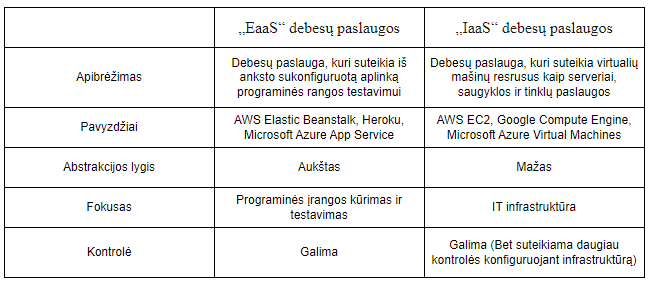
\includegraphics[scale=0.9]{img/EassvsIaas.png}
    \caption{„EaaS“ ir „IaaS“ metodikų palyginimas}
    \label{img:mlp}
\end{figure}

\subsection{Laikinųjų aplinkų skirtumai nuo statinių}

Laikinosios aplinkos (dar kitaip vadinamos peržiūros aplinkomis) yra skirtos testuoti konkretaus funkcionalumo ar šakos kodą prieš vykdant naują leidimą į produkcinę aplinką \cite{SaltVienuoliktas}. Skirtingai nuo įprastų (statinių) aplinkų, kurias aptarėm „Git“ šakojimosi strategijų skyriuje, šios yra naudojamos konkrečiam tikslui, o jį įgyvendinus ištrinamos. Taip išvengiama tokių problemų, kaip duomenų perkrova vienoje aplinkoje bei sunkesnio klaidų vietos identifikavimo, kai keli nauji funkcionalumai yra pasiekę kokybės užtikrinimo aplinką. Taip pat laikinosios aplinkos reikalauja ir struktūrinių pakitimų procesuose, kad verifikacijos dalis būtų vykdoma prieš suliejant šakos kodą į kažkurią iš aplinkų. Šie pokyčiai yra būtini, nes peržiūros aplinkų paskirtis yra izoliuoti likusius kodo pakitimus nuo kitų bei paruošti konkrečios šakos aplinką. Testavimo procesas tampa dar labiau automatizuotas bei patikimas, nes pasinaudojant „EaaS“ debesų kompiuterijos paslaugą yra inicijuojama laikinoji aplinka ir programuotojams tam nereikia skirti jokio papildomo laiko. Laikinųjų aplinkų efektyvumą rodo ir 2022 metais įmonės „Uffizzi“ atliktas tyrimas, kuris teigia, kad integravus laikinųjų aplinkų sprendimą, leidimų dažnumas paaugo 64 procentais, o užduočių atlikimas per programuotoją tapo efektyvesnis 36 procentais \cite{SaltDvyliktas}.

\begin{figure}[H]
    \centering
    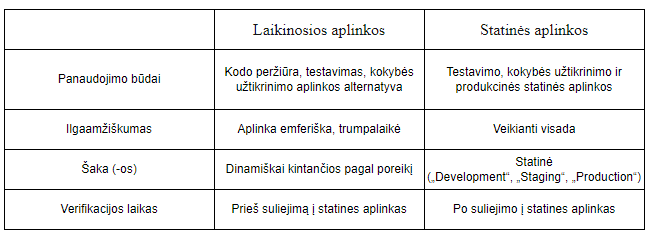
\includegraphics[scale=0.9]{img/LaikinosVsStatines.png}
    \caption{Laikinųjų ir statinių aplinkų palyginimas}
    \label{img:mlp}
\end{figure}

\subsection{„Git“ šakojimosi strategijų praplėtimas}

„Git“ šakojimosi strategijos yra vienas iš pagrindinių nepertraukiamo diegimo elementų, todėl norint į šį procesą įtraukti laikinąsias aplinkas yra reikalinga jas praplėsti ir pakoreguoti pagal prieš tai aptartus laikinųjų bei statinių aplinkų skirtumus. Labiau kompleksiniams metodams tai suteiks galimybę supaprastinti procesus su šio tipo aplinkomis, o greitiems metodams pagerinti kokybę ir verifikaciją. 

Tarp pagrindinių šiame darbe aptartų šakojimosi metodų - „GitFlow“ yra pats kompleksiškiausias, tačiau jo veikimo principas leidžia leidimus paruošti užtikrintai ir saugiai. Problemos su kuriomis susiduria šis metodas daugiausiai yra susiję su greičiu per kurį leidimas pasiekia produkcinę aplinką. Todėl integruojant laikinąsias aplinkas siekiama padidinti metodo efektyvumą. Galimi pokyčiai integravus laikinasias aplinkas: 

\begin{itemize}
  \item \textit{Kiekvieno funkcionalumo šaka testuojama su laikinosiomis aplinkomis}. Siekiant supaprastinti testavimo ir peržiūros procesus, kiekvienai kodo sujungimo užklausai galima naudoti laikinąsias aplinkas. Jos leistų programuotojams arba testuotojams, siekiantiems peržiūrėti kodą, turėti paruoštą aplinką be papildomų pastangų - tiek kliento pusės programą, tiek API serverius. Tai suteikia tinkamas sąlygas įsitikinti ar paruoštas funkcionalumas veikia tinkamai.

  \item \textit{Leidimo šakų atsisakymas ir jų pakeitimas laikinosiomis aplinkomis}. Vienas iš labiausiai kompleksiškumą sukuriančių šakų tipų yra „Release“, nes šios šakos yra reikalingos tik laikinam laiko periodui, kol yra nusprendžiama kodą sulieti su pagrindine produkcinės aplinkos kodo baze arba leidimas tampa pasenęs ir nebereikalingas. Todėl statinių šakų atsisakymas ir laikinų aplinkų naudojimas su kiekvienu kodo sujungimo prašymu (angl. \textit{Merge Request}) iš „Development“ tipo aplinkos į „Production“, leistų turėti identifikuotus leidimus bei neturėti pastovių aplinkų laikinumu pasižyminčiam komponentui.
  
  \item \textit{„Hotfixes“ šakų laikinosios aplinkos}. Vienas iš didžiausių trūkumų su greitų problemų sutvarkymo šakomis yra neturėjimas tarpinės erdvės, kurioje kodas būtų patestuojamas, nes yra reikalingas skubus problemos sprendimas. Tačiau laikinosios aplinkos pasižymi tuo, kad jos nereikalauja jokių papildomų pastangų. Dėl šios priežasties „Hotfixes“ šakos galėtų būti testuojamos pasitelkiant jas, taip užtikrinant, kad kodas patekęs į produkcinę aplinką veiks tinkamai.

\end{itemize}

Kiti du šiame darbe aptarti metodai yra „GitHub Flow“ ir „GitLab Flow“. Kadangi juose neegzistuoja „Hotfixes“ ir „Release“ tipo šakos - galimas tik kiekvieno funkcionalumo šakų testavimo su laikinosiomis aplinkomis pokytis. Jis suteikia šiems metodams daugiau užtikrintumo bei apsaugos, kadangi yra tiesiai suliejamas kodas į statines klientams arba užsakovams pasiekiamas aplinkas.

Tačiau „Trunk-based development“ metodas išvis neturi jokių papildomų šakų ir visas kodas yra parašytas bei rašomas vienoje pagrindinėje aplinkoje, dar kitaip vadinamoje kamienu (angl. \textit{trunk}). Vienintelis laikinųjų aplinkų panaudojimo būdas - sukurti automatizuotą sprendimą, kuris paruoštų aplinką konkrečiam pakeitimų įrašui (angl. \textit{commit}), kadangi šis metodas stokoja atskirtos kodo bazės tarp skirtingų funkcionalumų.


\subsection{Būdai integruoti metodiką}

Įmonėms norinčioms integruoti laikinųjų aplinkų metodiką reikia pasirinkti iš dviejų galimų būdų tai padaryti:

\begin{itemize}
  \item \textit{„EaaS“ tipo įrankių integracija su automatiniais procesais}. Paprastesnis yra šis metodas, kuris siūlo naudoti debesų kompiuterijos paslaugas, turinčias iš anksto paruoštą konfigūraciją ir reikalauja tik esminių detalių apie kuriamo produkto konteinerizuotas programas, kad būtų suteikta informacija kokiu būdu ir su kokiais poreikiais programinė įranga gali būti sėkmingai paruošta paslaugas suteikiančių kompanijų serveriuose. Tuomet seka integracija su įrankiais skirtais automatizuoti programinės įrangos procesus (tokie kaip „Github Actions“, „GitLab CI/CD“ ar kiti). Kiekvienas „EaaS“ sprendimas turi savo paleidimo būdus kaip paruošti, kad mūsų kiekviena nauja kodo sujungimo užklausa automatiškai paruoštų naują laikinąją aplinką.

  \item \textit{Savarankiškai paruoštas sprendimas}. Egzistuoja įvarių priežasčių dėl kurių įmonėms gali netikti jau egzistuojantys „EaaS“ tipo įrankiai - teisiniai reguliavimai, duomenų saugumas ir kiti. Šiuo atveju yra kuriamas sprendimas su įvairiais konteinerių orchestravimo įrankiais kaip „Kubernetes“, kai patys „DevOps“ specialistai ruošia automatizuotus procesus, kurie su kiekviena nauja kodo sujungimo užklausa ruošia laikinąją aplinką jų pačių debesų klasteriuose (angl. \textit{Cloud clusters}).

\end{itemize}

\begin{figure}[H]
    \centering
    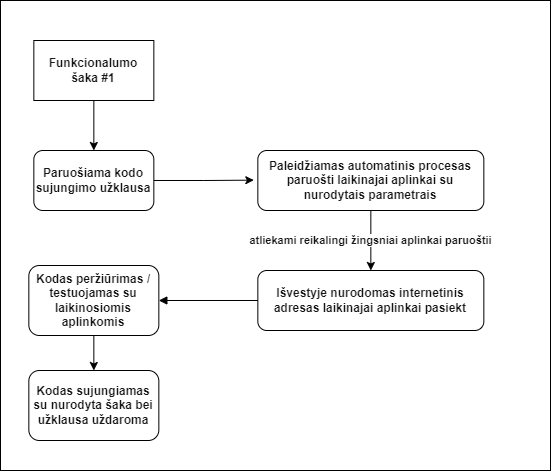
\includegraphics[scale=0.6]{img/PvzBuduv2.png}
    \caption{Integruoto laikinųjų aplinkų sprendimo pavyzdys}
    \label{img:mlp}
\end{figure}

\subsection{Apibendrinimas}

Laikinųjų aplinkų metodas papildo daugelį strategijų naudojamų programinės įrangos išleidimo valdymui internetinėms programoms. Pati metodika yra paremta debesų kompiuterijos paslaugos „EaaS“ principu, kai visa IT infrastruktūra yra sukonfigūruota iš anksto ir kiekvienam scenarijui, kai reikalingos laikinosios aplinkos, nebereikia rūpintis kaip debesų serveriuose programa bus paruošta naudojimui. Strategija išsiskiria tuo, kad yra priešingybė tradicinėms statinėms aplinkoms, nes veikia emferiškai, dinamiškai prisitaiko prie kodo pakeitimų. Norint pasiekti išvadų šiame darbe - svarbu integruoti laikinąsias aplinkas, kadangi nėra daug apibrėžiančių empirinių tyrimų, kaip tai tinkamai padaryti.

% TODO: Skyrius antroje dalyje apie issukius su laikinom aplinkoms (parodyt kaip sprest komplikacijas, jei iseina trecioje dalyje)

%  3 dalis. Praktinė dalis
\section{Laikinųjų aplinkų sprendimo integracija}

Siekiama įvykdyti laikinųjų aplinkų integraciją į pavyzdinį projektą, kurio kodas imituoja realios internetinės svetainės veikimą. Todėl bus naudojamas ir serverio pusės (angl. \textit{server-side}), ir į ją besikreipiančios vartotojo sąsajos programos, kad sukurti realų scenarijų. Pačiai laikinųjų aplinkų integracijai buvo pasirinktas rekomenduojamas įrankis pagal „Uffizzi“ produkto tyrimą, kuris buvo atliktas 2022 metais \cite{SaltDvyliktas}. Ši įmonė siūlo „EaaS“ tipo įrankį ir dokumentaciją, turinčią reikalingą informaciją apie integravimą. Jos tikslas yra parodyti, kad internetinėms svetainėms sprendimas veikia tinkamai ir kad nėra reikalinga jokia papildoma konfigūracija su kiekviena nauja kodo sujungimo užklausa. Visi automatizuoti procesai, konfigūracijos bei programinis kodas yra laikomas „GitHub“ platformoje.

\subsection{Pavyzdinis svetainės kodas}

Imituoti realios internetinės programos veikimui bus reikalingi du komponentai - serveris ir vartotojo sąsajos programa. Abiems naudoti pasirinkta „JavaScript“ programavimo kalba dėl savo paprastumo bei mažo kompleksiškumo, taip pat kliento aplikacijai reikalinga ir standartinė HTML  kompiuterinė žymėjimo kalba (žr. \hyperref[priedas1]{1} ir \hyperref[priedas2]{2} priedus). Svetainės veikimo principas bus toks: registruojamas kiekvienas mygtuko paspaudimas siunčiant į serverį per jungtį (angl. \textit{socket}) bei tiesiogiai atvaizduojama kiek tokių paspaudimų jau buvo.

\begin{figure}[H]
    \centering
    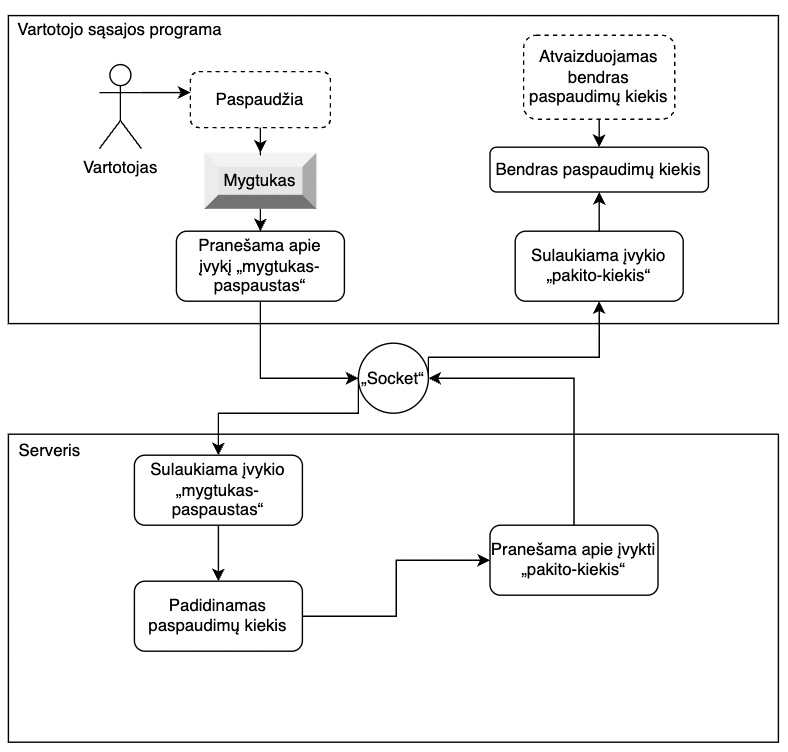
\includegraphics[scale=0.8]{img/Aplikacija.png}
    \caption{Pavyzdinės internetinės svetainės veikimas}
    \label{img:mlp}
\end{figure}

\subsection{Pasiruošimas programinės įrangos leidimams}

Aplikacijai sėkmingai veikiant reikia paruošti konteinerizuotas programas, kad programinė įranga veiktų vienodai, nepaisant to, kokiame serveryje šis kodas bus įdiegtas. Tai įgyvendintų pagrindinę sąlygą, kurią reikia išpildyti, siekiant turėti produkcinį programos variantą. „Docker“ platforma leidžia paruošti tokio tipo atvaizdus (angl. \textit{images}). Tiek serverio, tiek kliento pusės kodas yra ruošiamas ta pačia veiksmų seka, kuri aprašoma „Dockerfile“ tipo faile (žr. \hyperref[priedas3]{3 priedą}):

\begin{enumerate}
  \item Importuojamas oficialus „Node“ 16 versijos atvaizdas.
  \item Pasirenkama darbo direktorija kuriamame atvaizde.
  \item Įklijuojami konfigūracijos failai, kurie aprašo kokie paketai yra reikalingi.
  \item Įrašomi reikalingi paketai pagal konfigūraciją.
  \item Įklijuojamas likęs programinis kodas.
  \item Nurodoma atvaizdo paleidimo metu naudojama komanda, kuri pradeda vykdyti programinį kodą.
\end{enumerate}

Sukompiliuoti abiejų komponentų atvaizdai gali būti sėkmingai naudojami produkcinėje aplinkoje arba laikinosiose aplinkose, nes veiks vienodai nepriklausomai nuo sistemos, kurioje bus įdiegti.

\subsection{Laikinųjų aplinkų paruošimas naudojimui}

Su parašytu kodu bei paruoštomis konteinerių konfigūracijomis, ši programa turi esmines dalis, reikalingas programinės įrangos išleidimo valdymui. Tačiau norint turėti laikinąsias aplinkas su kiekviena šakos sujungimo užklausa, dar reikia papildomai atlikti keletą žingsnių.

    \subsubsection{Skirtingi integracijos būdai}

„Uffizzi“ įrankis įvertinant skirtingus įmonių poreikius suteikia du skirtingus būdus integruoti savo produktą \cite{SaltKeturioliktas}:

\begin{itemize}
  \item \textit{Integracija su „Github Actions“}. Šis sprendimas yra naudojamas, kai programinė įranga jau iš seniau turi savo paruoštą išleidimo valdymą bei automatinius „Github Actions“ procesus, kurie ruošia „Docker“ atvaizdus bei juos talpina į atitinkamus registrus. Tokiu atveju nėra atsisakoma šių procesų, o tik pridedami papildomi žingsniai integruojant „Uffizzi“ įrankį.

  \item \textit{Integracija su „Uffizzi CI“}. Produktui neturint jokio suformuoto išleidimo valdymo yra rekomenduojama naudoti šį būdą. Taip išvengiama automatizuotų procesų apsirašymo patiems „DevOps“ inžinieriams ir yra reikalinga tik „Docker Compose“ tipo konfigūracija, kuri apibrėžia mūsų programos komponentų poreikius.


\end{itemize}
    
Kadangi šio darbo imitacinė interneto svetainė dar neturi įgyvendintų automatizuotų procesų susijusių su išleidimu bei diegimu, integracija vyks naudojant „Uffizzi CI“.

    \subsubsection{Konfigūracija ir pasiruošimas integracijai}

Esminė konfigūracijos dalis - „Docker Compose“ tipo failas, kuris susideda iš reikalingų atvaizdų paruošimo parametrų bei nustatymų apie laikinųjų aplinkų gyvavimo ciklą ir trukmę \cite{SaltKeturioliktas}. Pagal parašytą programinį kodą (žr. \hyperref[priedas1]{1} ir \hyperref[priedas2]{2} priedus) - nėra reikalingi jokie aplinkų kintamieji (angl. \textit{environment variables}), tik nurodytas reikalingas prievadas (angl. \textit{port}) bei kur rasti „Dockerfile“ tipo failą kiekvienam iš komponentų. Po to yra nurodomi laikinųjų aplinkų parametrai:

\begin{itemize}
  \item Diegti laikinąją aplinką, kai kodo sujungimo užklausa atidaroma - laikinoji aplinka automatiškai paruošiama.

  \item Ištrinti laikinąją aplinką, kai kodo sujungimo užklausa uždaroma - laikinoji aplinka panaikinama.

  \item Kai laikinoji aplinka paruošiama - parašomas išvesties pranešimas kodo sujungimo užklausoje apie internetinį adresą, kuriame veikia laikinoji aplinka bei kur galima peržiūrėti jos statusą.
  
\end{itemize}

Tačiau „Uffizzi“ sprendimas suteikia tik vieną internetinės svetainės subdomeną visai aplinkai, ko pasekoje yra reikalingas apkrovos išlygintuvas (angl. \textit{load balancer}), kuris pagal užklausą nukreipia į atitinkamą komponentą - arba kliento pusės aplikaciją, arba serverį. Panaudojus populiaraus apkrovos išlygintuvo įrankio „Nginx“ oficialų „Docker“ atvaizdą paruošiamas „Dockerfile“, kuriame įkeliama konfigūracija apibrėžianti kur kokios užklausos turėtų būti nukreipiamos (žr. \hyperref[priedas5]{5 priedą}). Visi kreipimaisi į jungties serverį bus nukreipiami į serverį, o likę į kliento pusės programą.

Galiausiai darbe grįžtasma prie pagrindinės konfigūracijos. Pridedamas apkrovos išlygintuvas nurodant, kad laikinosios aplinkos vienintelis subdomenas bus nukreiptas į jį (žr. \hyperref[priedas6]{6 priedą}).

% TODO: Pridėti lb schemukę

    \subsubsection{„Uffizzi CI“ prijungimas}

Įvardinus mūsų programinės įrangos poreikius laikinosiose aplinkose, belieka tik duoti leidimą „Uffizzi CI“ įrankiui priėjimą prie produkto repozitorijos bei pateikti „Docker Compose“ konfigūracijos failo vietą. Sulig šiais veiksmais ne ilgiau nei po 5 minuičų kiekviena kodo sujungimo užklausa gauna nuorodą į veikiančią laikinąją aplinką (žr. \hyperref[priedas6]{6 priedą}). Taip pat, suteikiama galimybė per „Uffizzi CI“ platformą stebėti kiekvieno atvaizdo žurnalus (angl. \textit{logs}), stebėti kiekvieno komponento būseną ir klaidas, jei tokios nutiko. Visa tai įmanoma dėl prižiūrėtų automatinių procesų ir „EaaS“ metodikos, kuri suteikia reikiamą IT infrastruktūrą be jokių papildomų inžinierių pastangų.

\begin{figure}[H]
    \centering
    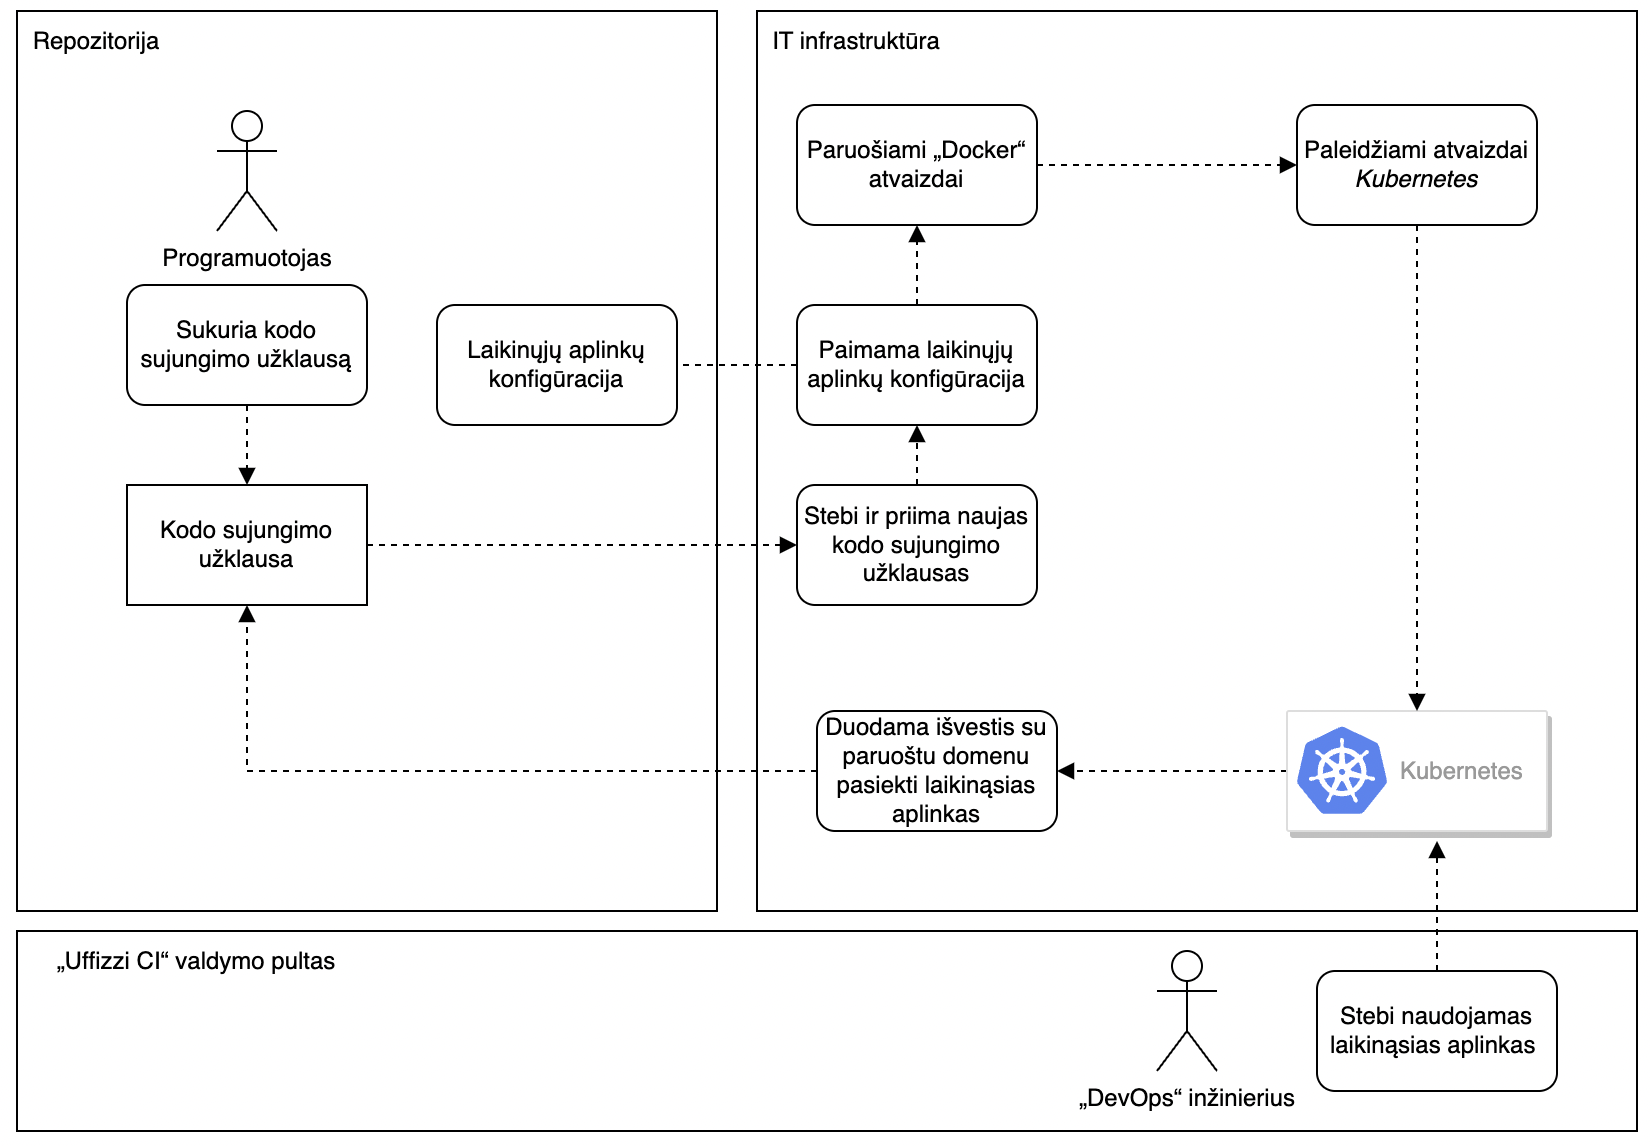
\includegraphics[scale=0.55]{img/Veikimas.png}
    \caption{Įgyvendinto „Uffizzi CI“ laikinųjų aplinkų sprendimo schema}
    \label{img:mlp}
\end{figure}

\subsection{Apibendrinimas}

Imituotai internetinei programai pavyko pritaikyti vieną iš rekomenduojamų laikinųjų aplinkų sprendimą, kuris nereikalavo iš anksto paruošto programinės įrangos išleidimo su registrais paruoštiems atvaizdams. Kodo sujungimo užklausos tapo paprasčiau peržiūrimos, nes nėra reikalingi rankiniai žingsniai tam pasiekti. Taip pat įrankis suteikė „DevOps“ inžinieriams patogų valdymo pultą, skirta stebėti bei valdyti šiuo metu veikiančias laikinąsias aplinkas. Tačiau netgi ir jau iš anksčiau naudojant tradicinį programinės įrangos išleidimo valdymą, šį sprendimą būtų galima pritaikyti pagal poreikius, nes konfigūracija suteikia pakankamai parametrų tiems dalykams apibrėžti.

\sectionnonum{Rezultatai ir išvados}

Darbo metodu pasiekti \textbf{rezultatai}:

\begin{enumerate}
  \item Išanalizuoti tradiciniai programinės įrangos išleidimo internetinėms programoms būdai.
    \begin{itemize}
      \item Įvardinti baziniai principai, kuriais vadovaujantis susiformavo programinės įrangos išleidimo valdymas.
      \item Apžvelgtos „Agile“ ir „Lean“ metodikų sąvybės, kurios atsispindi tradciniam leidimų valdyme.
      \item Apibrėžta „DevOps“ pozicijos ir automatizacijos svarba siekiant efektyvių leidimų.
      \item Paaiškintos skirtingos „Git“ šakojimosi strategijos leidimų valdyme
    \end{itemize}
  \item Apžvelgtas laikinųjų aplinkų sprendimas tokio tipo sistemoms bei jo taikymo būdai.
    \begin{itemize}
      \item Apibrėžta debesų kompiuterijos paslauga „EaaS“ ir jos panaudojimas su laikinosiomis aplinkomis.
      \item Palygintos laikinosios ir statinės aplinkos, įvardinant skirtumus.
      \item Praplėstos „Git“ šakojimosi strategijos integruojant ir laikinąsias aplinkas.
      \item Įvardinti skirtingi galimi būdai internetinėms programoms integruoti tokio tipo sprendimą.
    \end{itemize}
  \item Integruotas vienas iš laikinųjų aplinkų sprendimų į programinės įrangos išleidimo valdymą.
    \begin{itemize}
      \item Suprojektuotas ir suprogramuotas pavyzdinis svetainės kodas.
      \item Imitacinė internetinė svetainė buvo paruošta programinės įrangos leidimams „Docker“ platformos pagalba. 
      \item Pasirinktas integracijos tipas bei paruošta konfigūracija peržiūros aplinkom įgyvendinti.
      \item Sėkmingai įjungtos bei patestuotos laikinosios aplinkos su kiekviena nauja kodo sujungimo užklausa.
    \end{itemize}
\end{enumerate}

Darbo metodu padarytos \textbf{išvados}:

\begin{enumerate}
  \item Tradiciniai programinės įrangos išleidimo valdymo metodai užtikrina reikiamą saugumą ar greitį, tačiau susiduriama su problemomis, kai pasirinkus saugesnį metodą nukenčia greitis, o pasirinkus greitį, nukenčia saugumas.
  \item Laikinosios aplinkos keičia įmonėje vykdomų procesų eigą, nes kodo verifikacijos laikas yra daromas prieš suliejant kodą į statines aplinkas.
  \item Laikinųjų aplinkų integracija reikalauja papildomų pastangų bei priežiūros, todėl jų suteikiama nauda nėra vienareikšmiškai tik teigiama.
  \item Laikinosios aplinkos palengvina kodo peržiūros procesą, nes nėra reikalingi rankiniai žingsniai peržiūrėti veikiančią internetinę aplikaciją.
\end{enumerate}

\sectionnonum{Tolimesni darbai}
 
Siūloma dėl empirinių tyrimų trūkumo šiai temai atlikti tyrimą, kuris apibrėžtų pagrindines problemas pasirinkus šią strategiją, kokie taikymo būdai veikia geriausiai ir nustatytų kokybės bei kaštų santykį. Taip pat, svarbu šią programinės įrangos išleidimo metodiką nagrinėti toliau su labiau kompleksinėm architektūrom, kurios įtrauktų mikroservisus, duomenų bazes, vidinius tinklus ir kitas aplinkybės, apsunkinančiais laikinųjų aplinkų integraciją.

% TODO: Peržiūrėti, kad nebūtų piratuotų straipsnių link'ų
\printbibliography[heading=bibintoc,category=cited] % Šaltinių sąraše nurodoma panaudota
% literatūra, kitokie šaltiniai. Abėcėlės tvarka išdėstomi darbe panaudotų
% (cituotų, perfrazuotų ar bent paminėtų) mokslo leidinių, kitokių publikacijų
% bibliografiniai aprašai.  Šaltinių sąrašas spausdinamas iš naujo puslapio.
% Aprašai pateikiami netransliteruoti. Šaltinių sąraše negali būti tokių
% šaltinių, kurie nebuvo paminėti tekste.

% \sectionnonum{Sąvokų apibrėžimai}
% \sectionnonum{Santrumpos}
% Sąvokų apibrėžimai ir santrumpų sąrašas sudaromas tada, kai darbo tekste
% vartojami specialūs paaiškinimo reikalaujantys terminai ir rečiau sutinkamos
% santrumpos.

\appendix  % Priedai
% Prieduose gali būti pateikiama pagalbinė, ypač darbo autoriaus savarankiškai
% parengta, medžiaga. Savarankiški priedai gali būti pateikiami ir
% kompaktiniame diske. Priedai taip pat numeruojami ir vadinami. Darbo tekstas
% su priedais susiejamas nuorodomis.

\section{Serverio dalies programinis kodas}
\label{priedas1}
\begin{figure}[H]
    \centering
    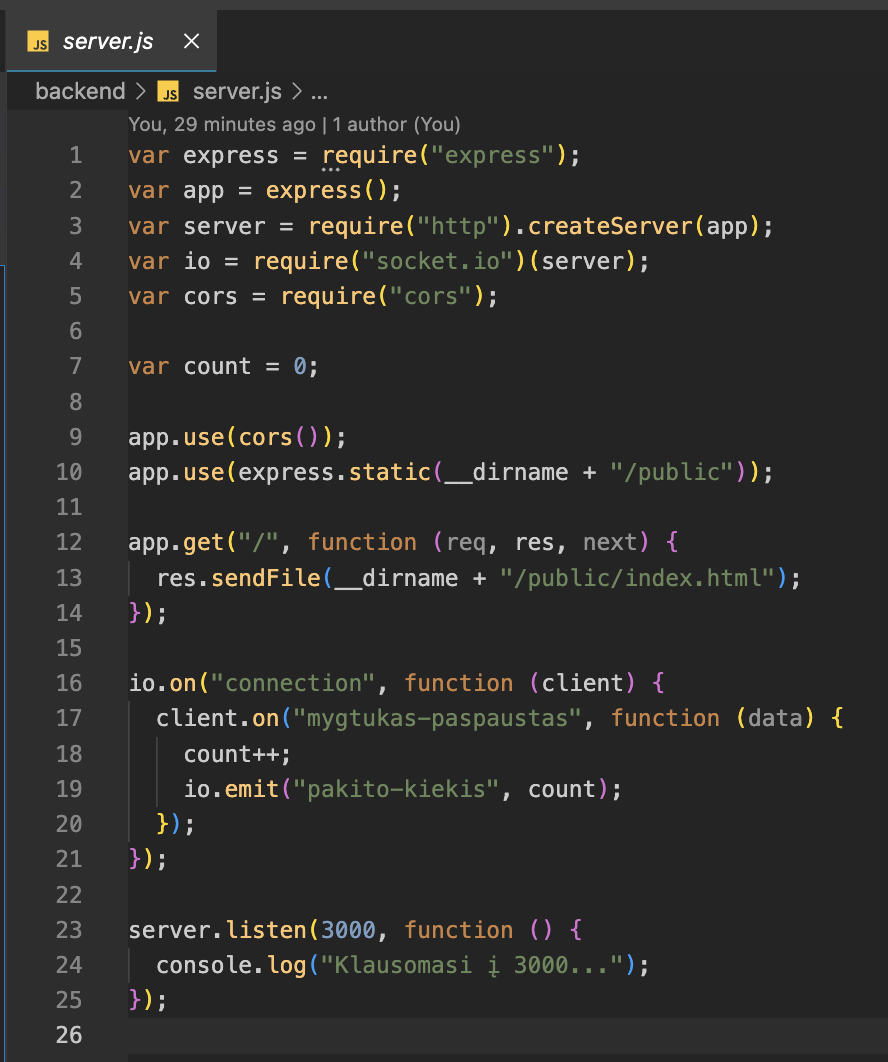
\includegraphics[scale=0.7]{img/priedai/backend-kodas.png}
    \caption{Serverio dalies programinis kodas}
    \label{img:mlp}
\end{figure}


\section{Vartotojo sąsajos dalies programinis kodas}
\label{priedas2}
\begin{figure}[H]
    \centering
    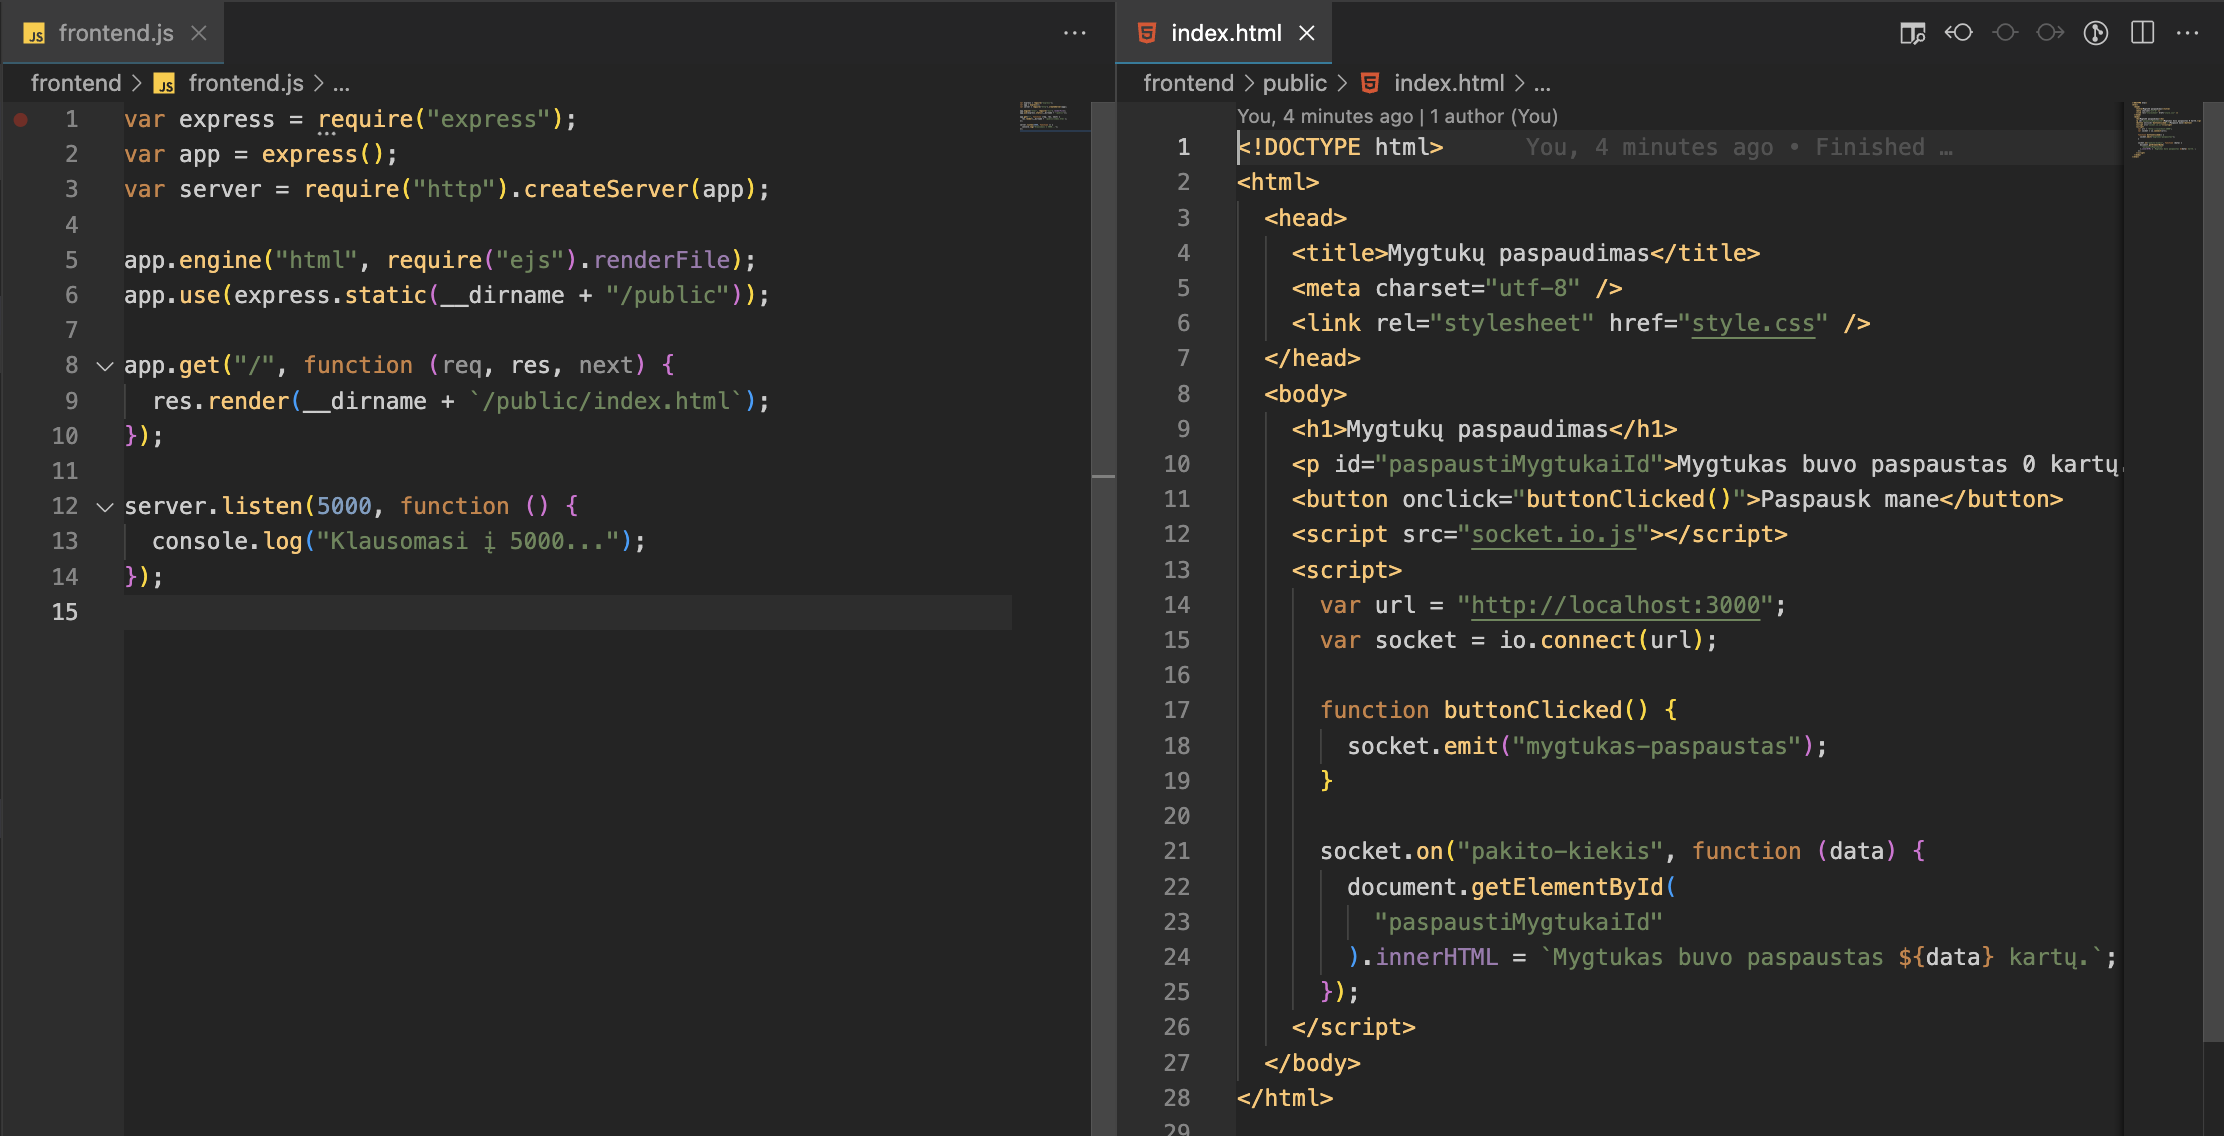
\includegraphics[scale=0.45]{img/priedai/frontend-kodas.png}
    \caption{Vartotojo sąsajos dalies programinis kodas}
    \label{img:mlp}
\end{figure}

\section{„Docker“ atvaizdų konfigūracija}
\label{priedas3}
\begin{figure}[H]
    \centering
    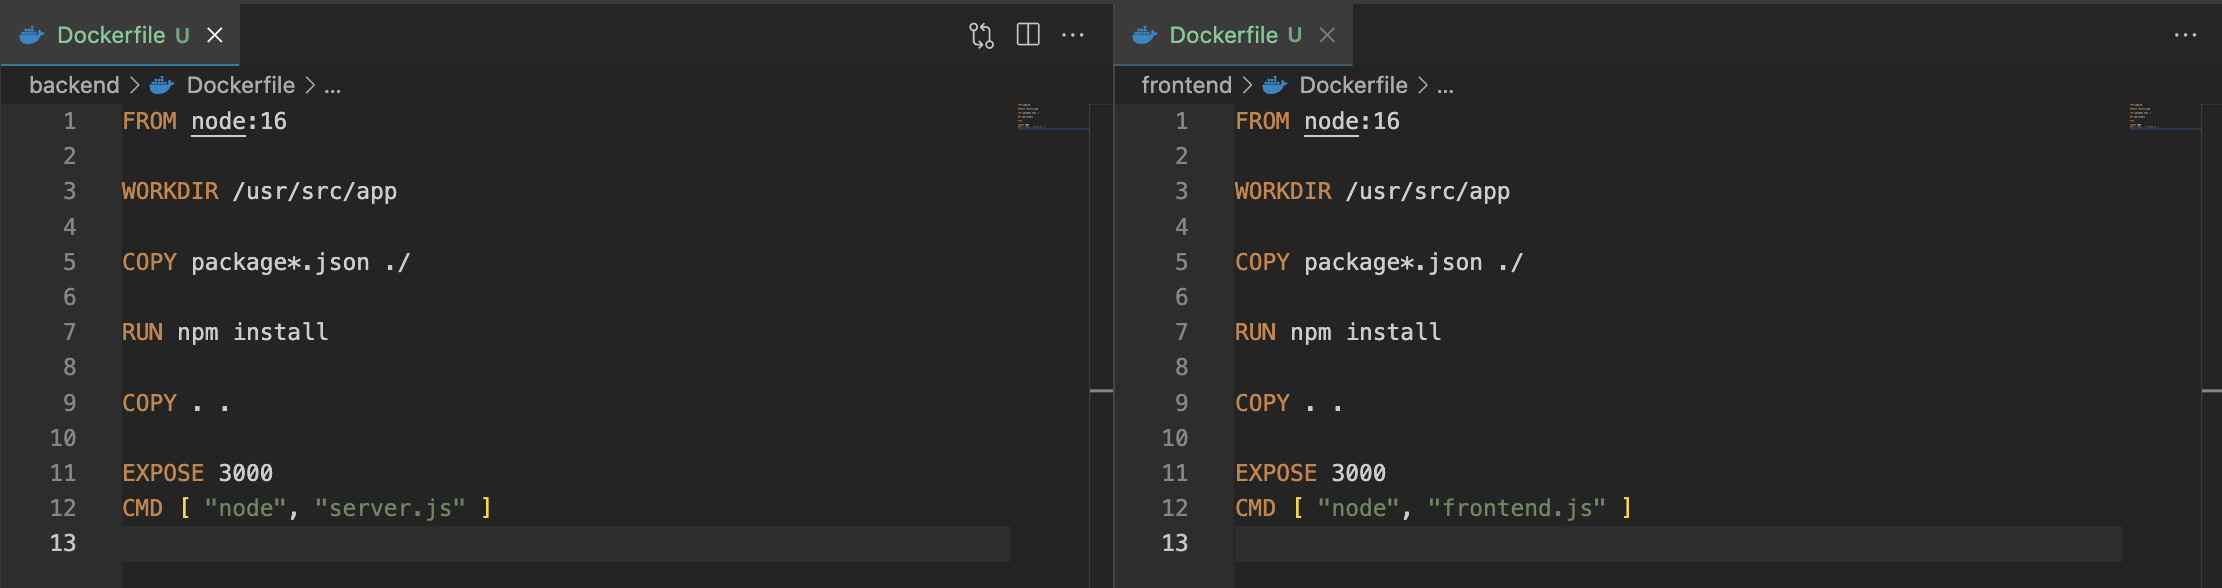
\includegraphics[scale=0.45]{img/priedai/dockerfiles.png}
    \caption{„Docker“ atvaizdų konfigūracija internetinės programos komponentams}
    \label{img:mlp}
\end{figure}

\section{„Nginx“ atvaizdo ir veikimo konfigūracijos}
\label{priedas4}
\begin{figure}[H]
    \centering
    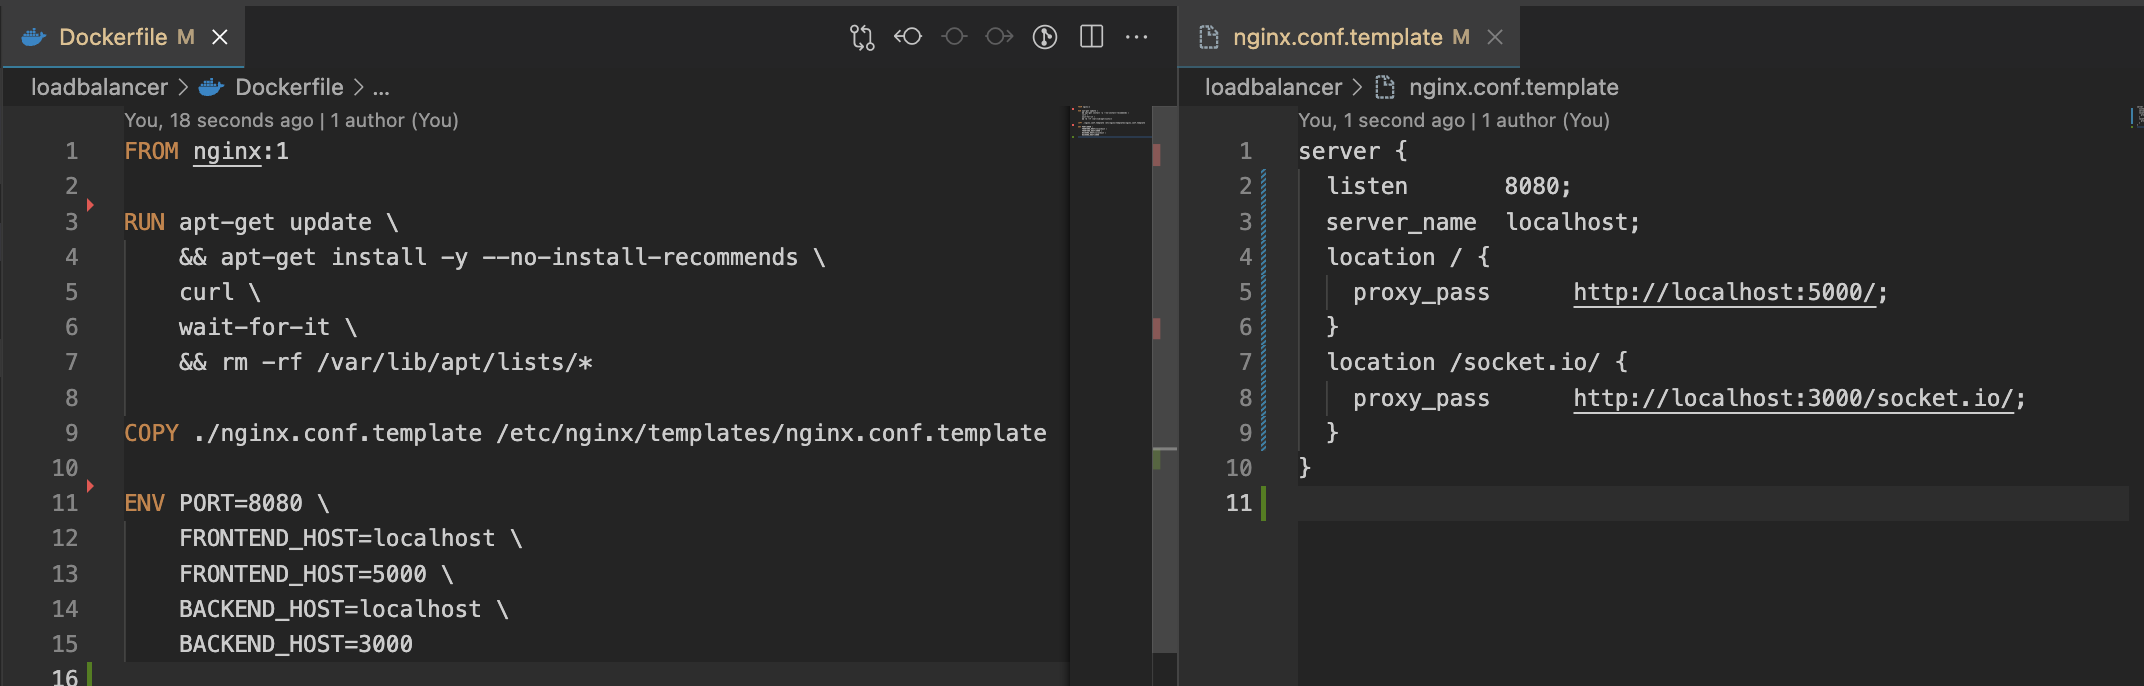
\includegraphics[scale=0.45]{img/priedai/nginx.png}
    \caption{„Nginx“ atvaizdo ir veikimo konfigūracijos}
    \label{img:mlp}
\end{figure}

\section{Laikinųjų aplinkų konfigūracija}
\label{priedas5}
\begin{figure}[H]
    \centering
    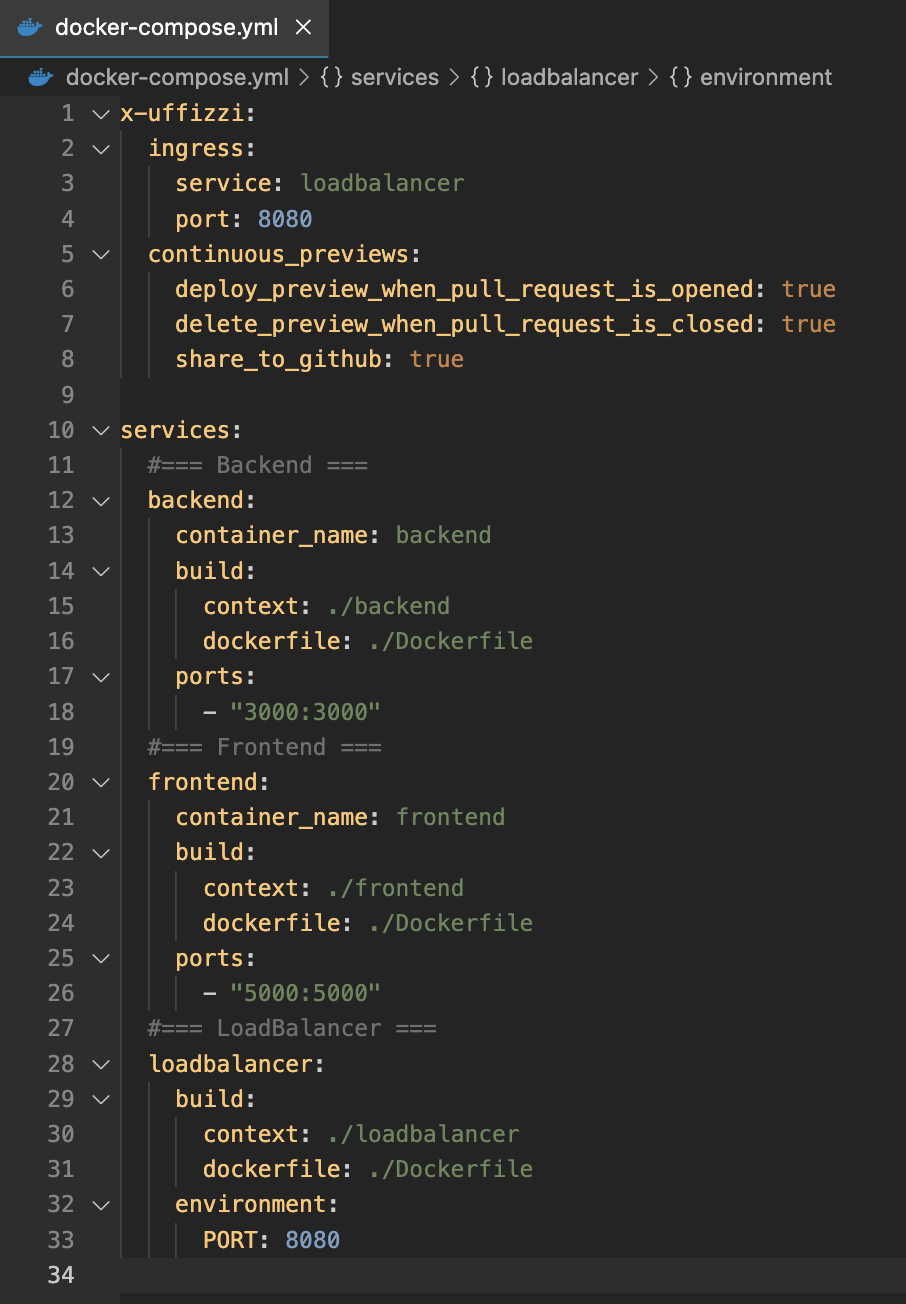
\includegraphics[scale=0.7]{img/priedai/compose.png}
    \caption{Laikinųjų aplinkų konfigūracija}
    \label{img:mlp}
\end{figure}

\section{Ekrano nuotrauka rodanti laikinųjų aplinkų veikimą}
\label{priedas6}
\begin{figure}[H]
    \centering
    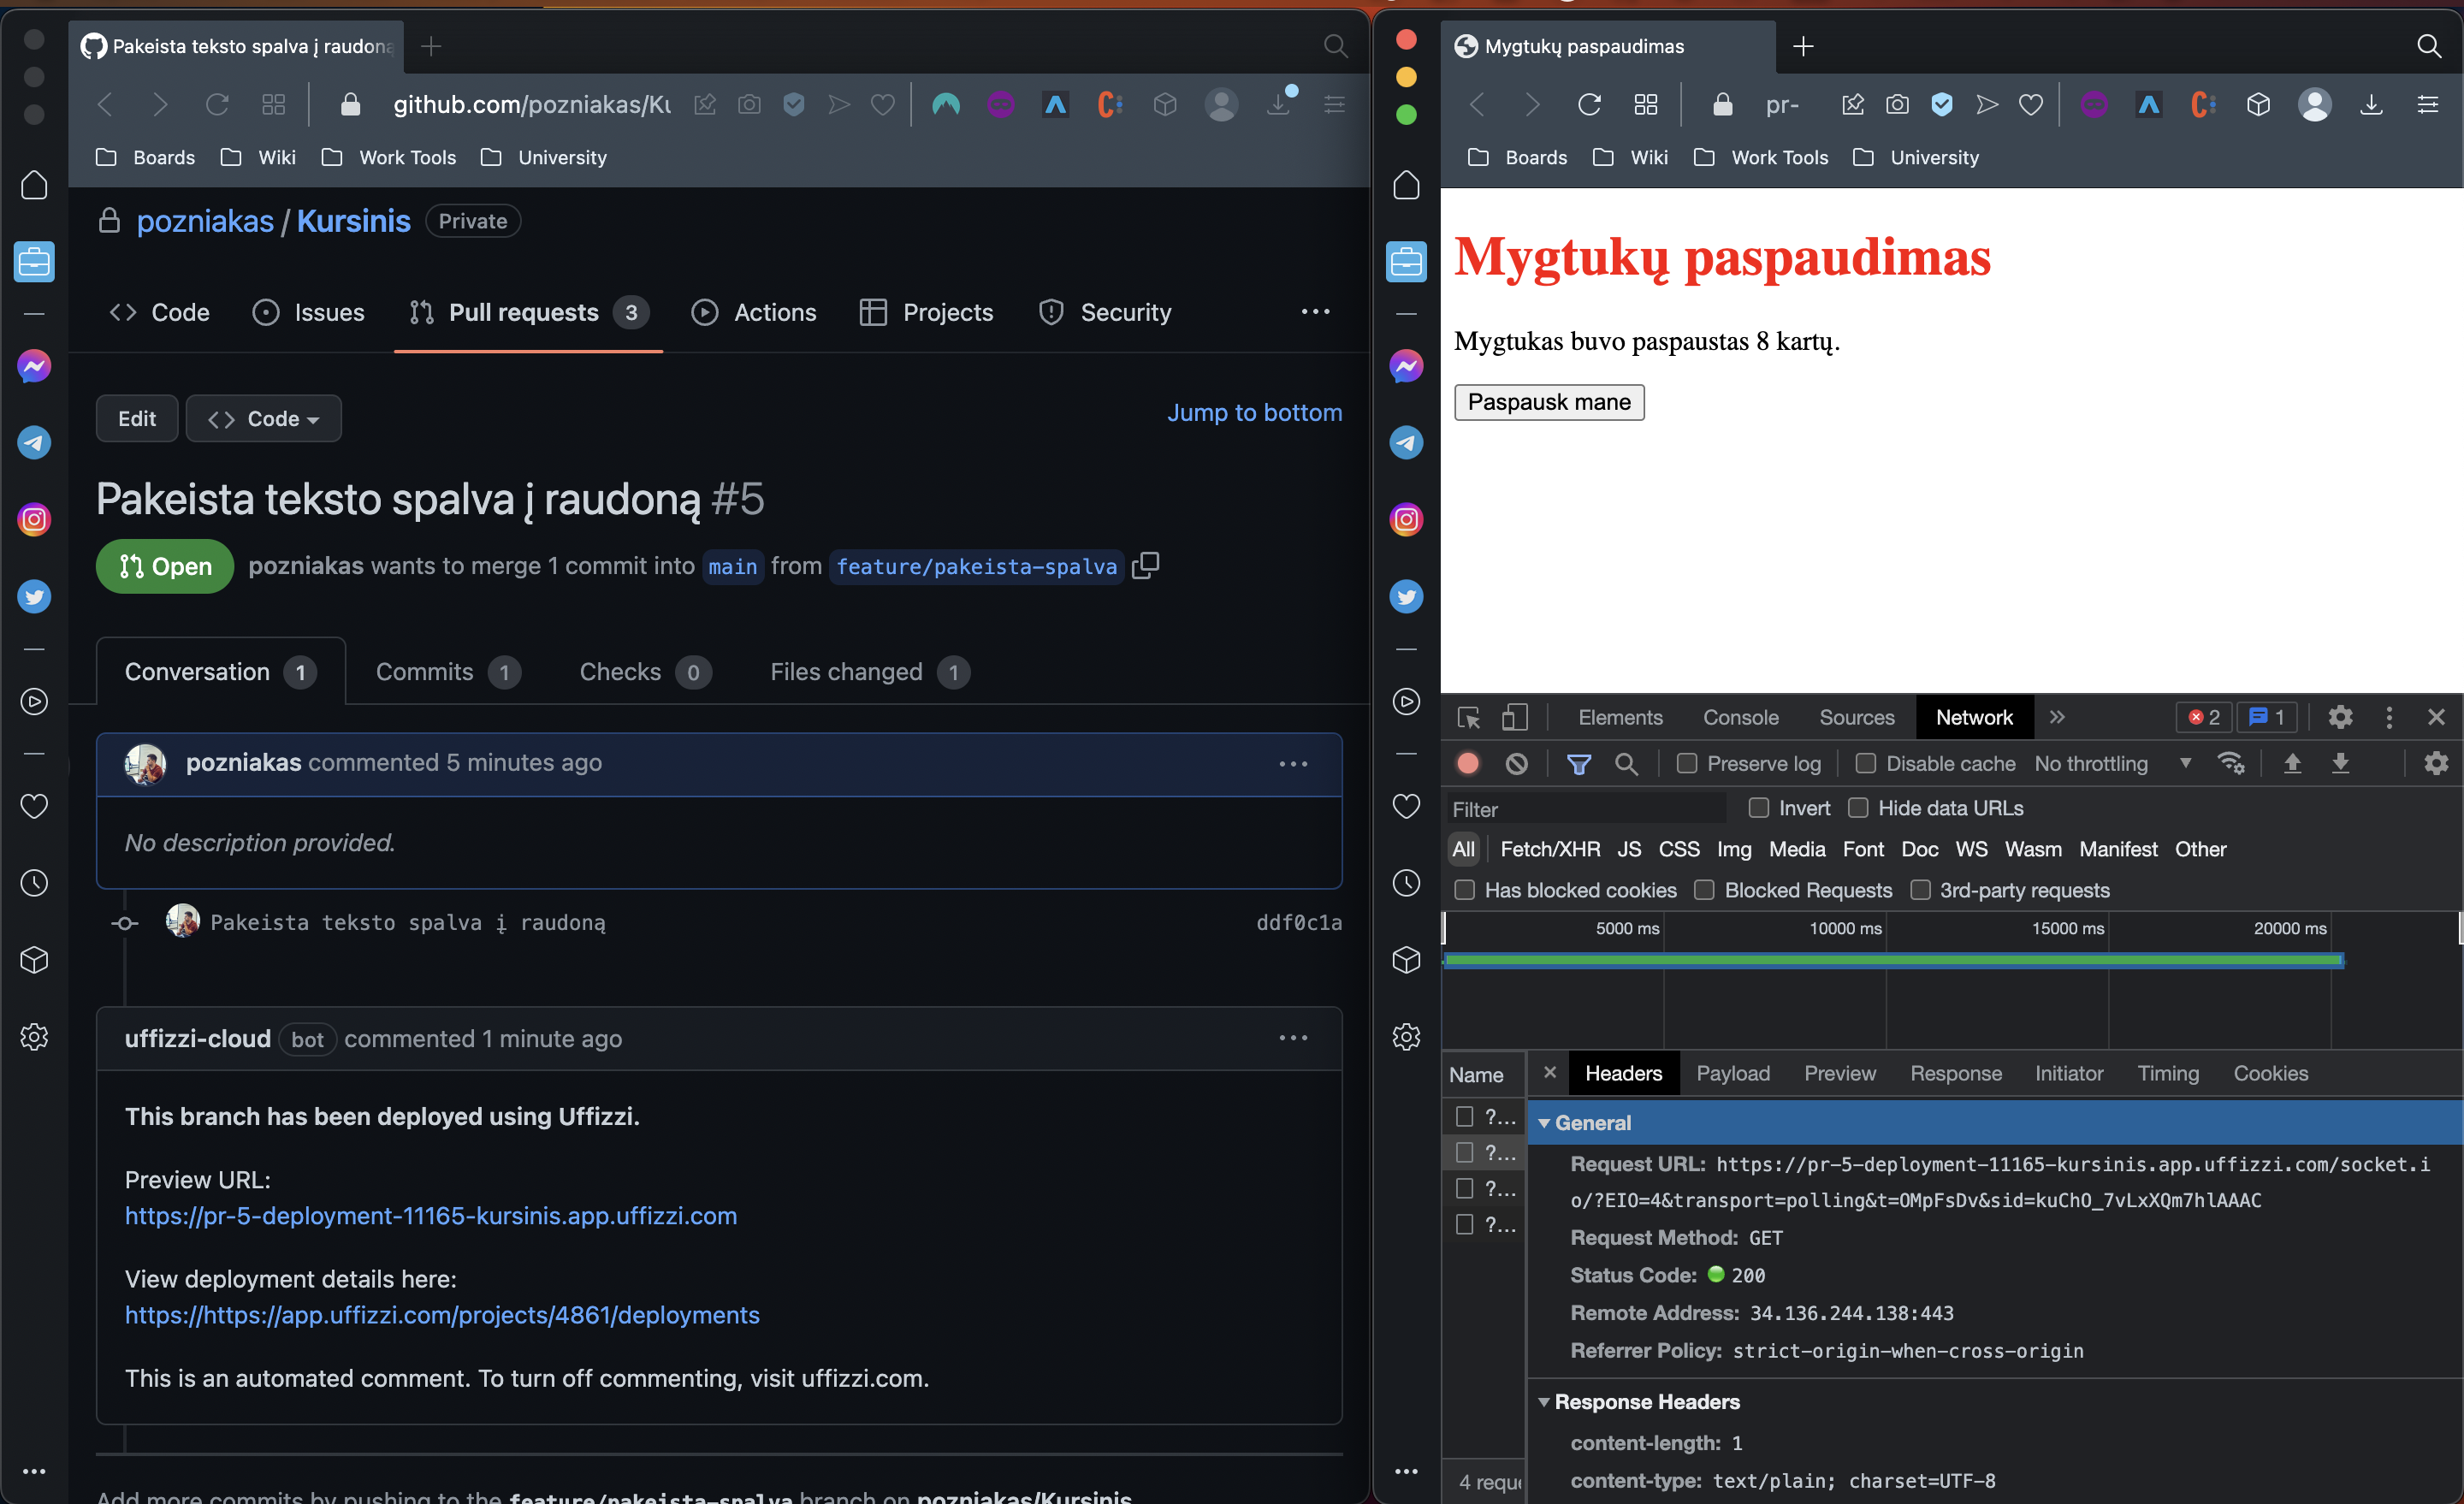
\includegraphics[scale=0.3]{img/Final.png}
    \caption{Ekrano nuotrauka rodanti laikinųjų aplinkų veikimą}
    \label{img:mlp}
\end{figure}

\end{document}

% TODO: Perdaryti pav i lenteles
% TODO: Išsiaiškinti apie priedų numeracijas
% TODO: Išsiaiškinti dėl literatūros, ar tinkamai aprašiau